%Este trabalho está licenciado sob a Licença Atribuição-CompartilhaIgual 4.0 Internacional Creative Commons. Para visualizar uma cópia desta licença, visite http://creativecommons.org/licenses/by-sa/4.0/deed.pt_BR ou mande uma carta para Creative Commons, PO Box 1866, Mountain View, CA 94042, USA.

\chapter{Derivação}\label{cap_deriv}
\thispagestyle{fancy}

Neste capítulo, discutimos os métodos fundamentais de derivação numérica de funções. A derivada de uma função $f$ num ponto $x$ é, por definição,
\begin{equation}
  f'(x) = \lim_{h\to 0} \frac{f(x+h) - f(x)}{h}.
\end{equation}
Assim sendo e assumindo $h>0$ próximo de zero, temos que $f'(x)$ pode ser aproximada pela razão fundamental, i.e.
\begin{equation}\label{eq_razao_fundamental}
  f'(x) \approx \underbrace{\frac{f(x+h) - f(x)}{h}}_{D_hf(x)}.
\end{equation}
Analisando a Figura~\ref{fig:intro_deriv} vemos que, geometricamente, isto é análogo a aproximar a declividade da reta tangente ao gráfico da função $f$ no ponto $(x,f(x))$ pela declividade da reta secante ao gráfico da função $f$ pelos pontos $(x,f(x))$ e $(x+h,f(x+h))$.

\begin{figure}[h]
  \centering
  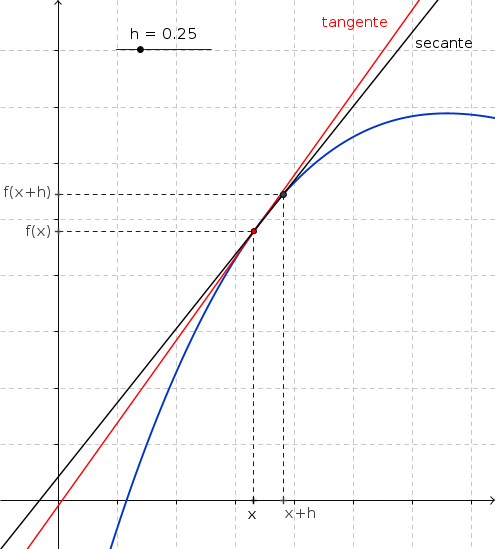
\includegraphics[width=0.7\textwidth]{cap_deriv/dados/fig_intro_deriv/fig_intro_deriv}
  \caption{Interpretação geométrica da aproximação da derivada pela razão fundamental. Veja no \href{https://github.com/phkonzen/notas/blob/master/src/MatematicaNumerica/cap_deriv/dados/fig_intro_deriv/fig_intro_deriv.ggb}{Geogebra}.}
  \label{fig:intro_deriv}
\end{figure}

\begin{ex}\label{ex_intro_deriv}
  A derivada de $f(x) = \sen(x)$ no ponto $pi/3$ é $f'(\pi/3) = \cos(\pi/3)=0,5$. Agora, usando a aproximação pela razão fundamental~\eqref{eq_razao_fundamental}, temos
  \begin{align}
    f'\left(\frac{\pi}{3}\right) \approx D_hf(x) &= \frac{f\left(\frac{\pi}{3}+h\right)-f\left(\frac{\pi}{3}\right)}{h}\\
          &= \frac{\sen\left(\frac{\pi}{3}\right)-\sen\left(\frac{\pi}{3}\right)}{h}. 
  \end{align}
Na Tabela~\ref{tab:ex_intro_deriv} temos os valores desta aproximação para diferentes escolhas de $h$.

\begin{table}[h]
  \centering
  \begin{tabular}{l|c|c}
    $h$ & $Df(\pi/3)$ & $|f'(\pi/3)-Df(\pi/3)|$\\ \hline
    $10^{-1}$ & $4,55902\E-1$ & $4,4\E-2$ \\
    $10^{-2}$ & $4,95662\E-1$ & $4,3\E-3$ \\
    $10^{-3}$ & $4,99567\E-1$ & $4,3\E-4$ \\
    $10^{-5}$ & $4,99996\E-1$ & $4,3\E-6$ \\
    $10^{-10}$ & $5.00000\E-1$ & $4,1\E-8$ \\\hline
  \end{tabular}
  \caption{Valores aproximados da derivada de $f(x)=\sen(x)$ no ponto $x=\pi/6$ usado a expressão~\eqref{eq_razao_fundamental}.}
  \label{tab:ex_intro_deriv}
\end{table}
\end{ex}

Ao longo deste capítulo, veremos outras formas para aproximar a derivada de funções. Também, discutiremos sobre estimativas de precisão das aproximações, entre outros aspectos.

\section{Derivadas de primeira ordem}

\emconstrucao